\begin{explanationbox}
\par\par\medskip
\begin{minipage}{\linewidth}
\noindent
\textbf{\textcolor{CExplanation}{一句话直觉}}\par\nobreak\smallskip
\par\noindent\textbf{两个端点的纵坐标以 $y_0$ 为中心，一高一低；抛物线的横坐标是纵坐标的平方。}两端点一作差，平方差立刻留下“和”，而“和”恰好是 $2y_0$。\par
\end{minipage}
\par

\par\medskip
\begin{minipage}{\linewidth}
\noindent
\textbf{\textcolor{CExplanation}{先从圆看懂：为什么要相减、为什么要相加？}}\par\nobreak\smallskip
\par
\begin{minipage}{\linewidth}
\begin{center}
\resizebox{0.78\linewidth}{!}{% 解析坐标严格确定：圆 x^2+y^2=25，A=(3,4), B=(3,-4), M=(3,0)
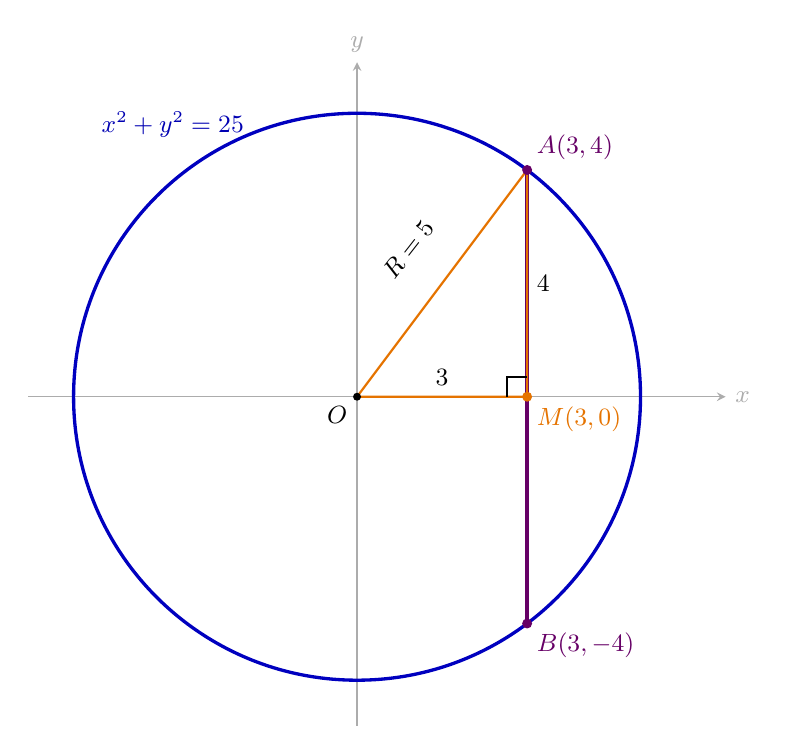
\begin{tikzpicture}[scale=.72,>=stealth,font=\small]
  \draw[->,gray!65] (-5.8,0)--(6.5,0) node[right] {$x$};
  \draw[->,gray!65] (0,-5.8)--(0,5.9) node[above] {$y$};
  \draw[very thick,blue!75!black] (0,0) circle (5);
  \draw[very thick,violet!80!black] (3,-4)--(3,4);
  \draw[thick,orange!90!black] (0,0)--(3,0)--(3,4)--cycle;
  \draw[black,thick] (2.65,0)--(2.65,.35)--(3,.35);
  \fill[black] (0,0) circle(2pt) node[below left] {$O$};
  \fill[orange!90!black] (3,0) circle(2.5pt) node[below right] {$M(3,0)$};
  \fill[violet!80!black] (3,4) circle(2.5pt) node[above right] {$A(3,4)$};
  \fill[violet!80!black] (3,-4) circle(2.5pt) node[below right] {$B(3,-4)$};
  \node[above] at (1.5,0.03) {$3$};
  \node[right] at (3,2.0) {$4$};
  \node[rotate=52] at (0.9,2.6) {$R=5$};
  \node[blue!70!black] at (-3.25,4.8) {$x^2+y^2=25$};
\end{tikzpicture}
}
\end{center}
\end{minipage}\par
\end{minipage}
\par

\par

圆 $x^2+y^2=R^2$ 上的弦设 $A=M+\mathbf v,\ B=M-\mathbf v$，其中
$M=(x_0,y_0)$，$\mathbf v=(u,t)$。把两点坐标分别代入圆的方程：
\[
\begin{aligned}
 (x_0+u)^2+(y_0+t)^2&=R^2,\\
 (x_0-u)^2+(y_0-t)^2&=R^2.
\end{aligned}
\]
\par\noindent\textbf{相减（方向）：}平方中的 $u^2,t^2$ 消掉，仅剩
\[
\boxed{x_0u+y_0t=0}
\quad\Longleftrightarrow\quad
\overrightarrow{OM}\cdot\overrightarrow{MA}=0.
\]
因此 $OM\perp AB$（$M\ne O$ 时确定唯一弦方向；$M=O$ 时各条直径都可）。
\par\noindent\textbf{相加（长度）：}混合项 $x_0u,y_0t$ 消掉，仅剩
\[
\boxed{x_0^2+y_0^2+u^2+t^2=R^2}
\ \Longleftrightarrow\ \boxed{OM^2+AM^2=R^2}.
\]
这才是真正的\textbf{勾股定理}：由于 $OM\perp AM$，直角三角形 $OMA$ 决定半弦长。
例如 $R=5$，$M=(3,0)$，相减得 $u=0$（竖直弦），相加得 $t^2=25-9=16$，所以 $A=(3,4),\ B=(3,-4)$，整弦长为 $8$。
\par\medskip
\begin{minipage}{\linewidth}
\noindent
\textbf{\textcolor{CExplanation}{再看抛物线：同一思路，另一种几何量}}\par\nobreak\smallskip
\par
\begin{minipage}{\linewidth}
\begin{center}
\resizebox{0.82\linewidth}{!}{% 精确数值：y²=4x, p=2, A(9,6), B(1,-2), M(5,2), T(1,2), 半位移 (u,t)=(4,4)
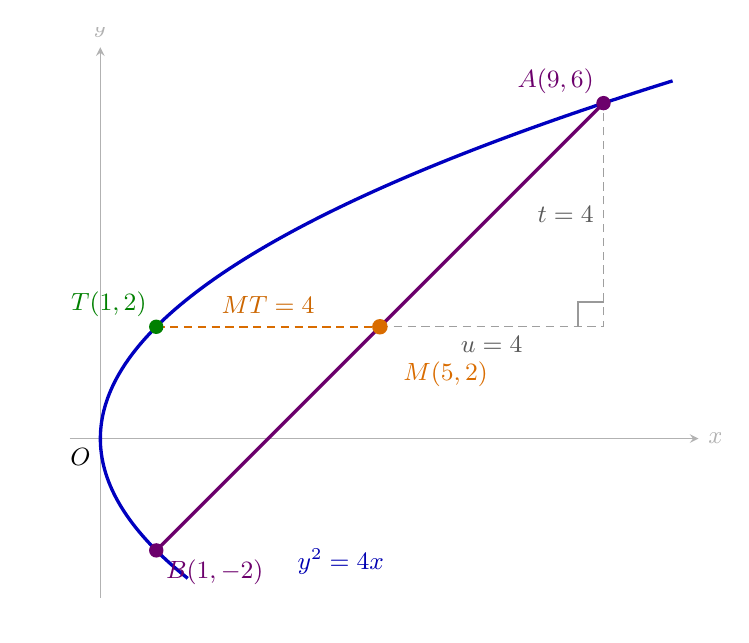
\begin{tikzpicture}[x=.71cm,y=.71cm,>=stealth,font=\small]
  \clip (-1.3,-3.15) rectangle (11.1,7.35);
  \draw[->,gray!60] (-.55,0)--(10.7,0) node[right] {$x$};
  \draw[->,gray!60] (0,-2.85)--(0,7.0) node[above] {$y$};
  \draw[blue!75!black,very thick,samples=125,domain=-2.5:6.4,variable=\v,smooth]
    plot ({\v*\v/4},{\v});
  \draw[violet!85!black,very thick] (1,-2)--(9,6);
  \draw[densely dashed,orange!85!black,thick] (1,2)--(5,2);
  \draw[gray!75,densely dashed] (5,2)--(9,2)--(9,6);
  \fill[violet!85!black] (9,6) circle (2.6pt) node[above left] {$A(9,6)$};
  \fill[violet!85!black] (1,-2) circle (2.6pt) node[below right] {$B(1,-2)$};
  \fill[orange!85!black] (5,2) circle (2.8pt) node[below right,xshift=5pt,yshift=-9pt] {$M(5,2)$};
  \fill[green!50!black] (1,2) circle (2.6pt) node[above left] {$T(1,2)$};
  \draw[gray!80,thick] (8.55,2)--(8.55,2.45)--(9,2.45);
  \node[above,orange!80!black] at (3.0,2.07) {$MT=4$};
  \node[below,gray!70!black] at (7.0,2) {$u=4$};
  \node[left,gray!70!black] at (9,4.0) {$t=4$};
  \node[blue!70!black] at (4.3,-2.2) {$y^2=4x$};
  \node[below left] at (0,0) {$O$};
\end{tikzpicture}
}
\end{center}
\end{minipage}\par
\end{minipage}
\par

\par

设 $A=(x_0+u,y_0+t)$、$B=(x_0-u,y_0-t)$，其中 $u,t$ 是\textbf{有符号半位移}，$t\ne0$。
\[
\begin{aligned}
 (y_0+t)^2&=2p(x_0+u),\\
 (y_0-t)^2&=2p(x_0-u).
\end{aligned}
\]
\par\noindent\textbf{相减（确定方向）：}把 $y_0^2$、$t^2$ 消去，只留下方向性很强的交叉项：
\[
4y_0t=4pu\quad\Longrightarrow\quad
\boxed{y_0t=pu}.
\]
因 $t$ 与 $u$ 同时给出半弦的竖、横分量，所以当 $y_0\ne0$ 时
$k=t/u=p/y_0$；当 $y_0=0$ 时，$u=0$，弦改为竖直。\textbf{“相减”正是在消去共同的弯曲量，留下位移方向。}

\par\noindent\textbf{相加（确定从中点走多远）：}消去 $y_0t$ 和 $pu$ 的交叉项，保留平方量：
\[
2y_0^2+2t^2=4px_0\quad\Longrightarrow\quad
\boxed{t^2=2px_0-y_0^2}.
\]
因此 $|t|=\sqrt{2px_0-y_0^2}$ 是\textbf{半弦的纵向展开量}；大于零才有不同实端点，等于零为切点，小于零无实弦。结合“相减”还可以恢复横向展开量
$u=y_0t/p$，从而确定整条弦的长度和端点。

\par\medskip
\begin{minipage}{\linewidth}
\noindent
\textbf{\textcolor{CExplanation}{抛物线的相加能不能叫勾股定理？}}\par\nobreak\smallskip
\par\noindent\textbf{不能直接这样叫。}令 $T=(y_0^2/(2p),y_0)$ 是曲线上与 $M$ \textbf{同纵坐标}的点。记有符号水平偏移 $x_0-x_T$，那么\par
\end{minipage}
\par

\[
\boxed{t^2=2p(x_0-x_T)}.
\]
对于真实弦，$p(x_0-x_T)>0$，所以改用实际长度 $MT=|x_0-x_T|$ 可写成
\[
\boxed{t^2=2|p|\,MT}.
\]

\par
\begin{minipage}{\linewidth}
\begin{center}
\begin{tikzpicture}[x=.95cm,y=.95cm,font=\small]
\path[use as bounding box] (-1,-1) rectangle (12,5.6);
\draw[fill=teal!12,teal!70!black,thick] (0,0) rectangle (3,3);
\node at (1.5,1.5) {$t^2=9$};
\node[below] at (1.5,0) {$|t|=3$};
\node[left] at (0,1.5) {$3$};
\node at (5,1.5) {$=$};
\draw[fill=orange!12,orange!85!black,thick] (7,0) rectangle (11,2.25);
\node at (9,1.1) {$2|p|\,MT=9$};
\node[below] at (9,0) {$2|p|=4$};
\node[right] at (11,1.1) {$MT=\frac94$};
\node at (5.5,4.7) {$y^2=4x,\quad M(\frac{13}{4},2),\quad T(1,2)$};
\node at (5.5,3.9) {相加给出等积关系；图中长度按同一比例绘制};
\end{tikzpicture}
\end{center}
\end{minipage}
\par

它表示\textbf{边长 $|t|$ 的正方形面积，等于以 $2|p|$ 和 $MT$ 为两边的矩形面积}；不是 $OM^2+AM^2=R^2$ 这样的勾股关系。
但最终求\textbf{实际半弦长}时，仍然能对水平分量 $u$ 与竖直分量 $t$ 使用真正的勾股定理：
\[
\boxed{AM^2=u^2+t^2
 =(2px_0-y_0^2)\!\left(1+\frac{y_0^2}{p^2}\right)}.
\]
\par\noindent\textbf{因此：圆的“相加”本身就是勾股；抛物线先“相加”得展开量，再与“相减”合并，用勾股求弦长。}
\par\medskip
\begin{minipage}{\linewidth}
\noindent
\textbf{\textcolor{CExplanation}{一加一减的统一原因：奇偶项分离}}\par\nobreak\smallskip
以中点为中心设成 $M\pm(u,t)$。\textbf{相减}时，含一次位移的奇项不互相抵消、平方位移的偶项抵消；\textbf{相加}则正相反。这不是凑技巧，而是曲线方程在中点两侧的\textbf{对称性}。\par
\end{minipage}
\par

\par\medskip
\begin{minipage}{\linewidth}
\noindent
\textbf{\textcolor{CExplanation}{最低门槛的理解（先给纵坐标）}}\par\nobreak\smallskip
设两端点纵坐标为 $y_0+t$、$y_0-t$（$t\ne0$）。由于 $x=y^2/(2p)$，\par
\end{minipage}
\par

\[
\underbrace{\Delta y}_{2t}=2t,\qquad
\underbrace{\Delta x}_{\text{平方差}/(2p)}
=\frac{(y_0+t)^2-(y_0-t)^2}{2p}
=\frac{2y_0t}{p}.
\]
因此 $\text{斜率}=\Delta y/\Delta x=p/y_0$。\textbf{只设 $t$ 一个未知量，不用解方程组。}
\par\medskip
\begin{minipage}{\linewidth}
\noindent
\textbf{\textcolor{CExplanation}{为什么没有 $x_0$？}}\par\nobreak\smallskip
$x_0$ 决定\textbf{弦有多长}，而 $y_0$ 决定\textbf{弦朝哪个方向}。由上面的对称设点可进一步得到\par
\end{minipage}
\par

\[
 x_0=\frac{y_0^2+t^2}{2p}
 \quad\Longleftrightarrow\quad
 t^2=2px_0-y_0^2.
\]
于是\textbf{有真实弦}必须且只需 $t^2>0$，即 $2px_0>y_0^2$。这也解释了：不能只凭 $k=p/y_0$ 就断言弦存在。
\par\medskip
\begin{minipage}{\linewidth}
\noindent
\textbf{\textcolor{CExplanation}{一个更深的几何联系（同纵标切线）}}\par\nobreak\smallskip
在曲线上另取 $T\bigl(y_0^2/(2p),y_0\bigr)$，即\textbf{纵坐标与中点相同的曲线点}，那么在 $y_0\ne0$ 时\par
\end{minipage}
\par

\[
 k_{\mathrm{tan},T}=\frac{p}{y_0}=k_{AB}.
\]
所以\textbf{中点弦平行于同纵标处的切线}，但 $M$ 通常不在曲线上，\textbf{不能误说“中点处的切线”}。此性质可由抛物线切线斜率 $\mathrm{d}y/\mathrm{d}x=p/y$ 得到，也可由点差法直接理解。
\par\medskip
\begin{minipage}{\linewidth}
\noindent
\textbf{\textcolor{CExplanation}{看到这些条件，立即想到什么？}}\par\nobreak\smallskip
\begin{itemize}[leftmargin=*,itemsep=0.4em]
 \item \textbf{已知弦中点 $M$、求弦方程：}先查 $2px_0>y_0^2$，再看 $y_0$ 是否为 $0$；最后用点斜式。
 \item \textbf{已知弦斜率 $k$、求中点的纵坐标：}直接 $y_0=p/k$；但只知道方向，不能唯一确定 $x_0$。
 \item \textbf{过定点的动弦、中点轨迹：}用“中点在动弦上”再结合 $k=p/y_0$ 消参；最后检查实交及竖直弦是否纳入。
\end{itemize}\par
\end{minipage}
\par

\par\medskip
\begin{minipage}{\linewidth}
\noindent
\textbf{\textcolor{CExplanation}{迁移提示}}\par\nobreak\smallskip
椭圆、双曲线的点差法往往同时带出 $x_0,y_0$；抛物线 $y^2=2px$ 因一次项只有 $x$，非竖直弦斜率只依赖 $y_0$。\par
\end{minipage}
\par

\end{explanationbox}
